\chapter{Introduction}

\section{Background of the Study}
\begin{itemize}
  \item Indian agriculture supports 600+ million farmers and contributes $\sim$17\% to national GDP.
  \item Government MSP procurement operates through thousands of procurement centers (mandis) across India.
  \item Farmers face severe inefficiencies at procurement centers:
    \begin{itemize}
      \item Uncontrolled physical queues stretching for kilometers.
      \item No visibility into wait times or slot availability before arrival.
      \item Manual procurement recording -- slow, error-prone, unaudited.
      \item Weeks of delay in payment with no tracking visibility.
      \item No digital communication channel between farmer and center.
    \end{itemize}
\end{itemize}

\section{Problem Statement}
\begin{itemize}
  \item No pre-booking system -- all farmers arrive simultaneously at peak hours.
  \item Physical queue is invisible -- farmers cannot see their position or wait time.
  \item Farmer, staff, and admin operate in information silos -- no unified platform.
  \item Post-procurement payment lifecycle is opaque and manually managed.
  \item No data-driven approach for predicting or balancing queue wait times.
\end{itemize}

\section{Objectives}
\begin{itemize}
  \item Build a full-stack, role-based web platform for Farmer, Staff, and Admin.
  \item Implement slot booking with capacity enforcement for procurement centers.
  \item Provide real-time live queue via Server-Sent Events (SSE) streaming.
  \item Integrate an ML-based wait time predictor (HistGradientBoosting, R\textsuperscript{2}~= 0.988).
  \item Enable digital procurement verification (weight, quality, rate, net payable).
  \item Build a complete payment lifecycle with settlement and dispute management.
  \item Deliver Web Push Notifications for real-time farmer alerts.
  \item Integrate an AI command agent (LangChain + Google Gemini) for NL queries.
\end{itemize}

\section{Overall System Architecture and Concept}
Figure~\ref{fig:project_overall} provides a comprehensive architectural and operational overview of the AgriQueue ecosystem.

\begin{figure}[htbp]
  \centering
  \fboxsep=0pt\relax
  {\color{gray!40}\fbox{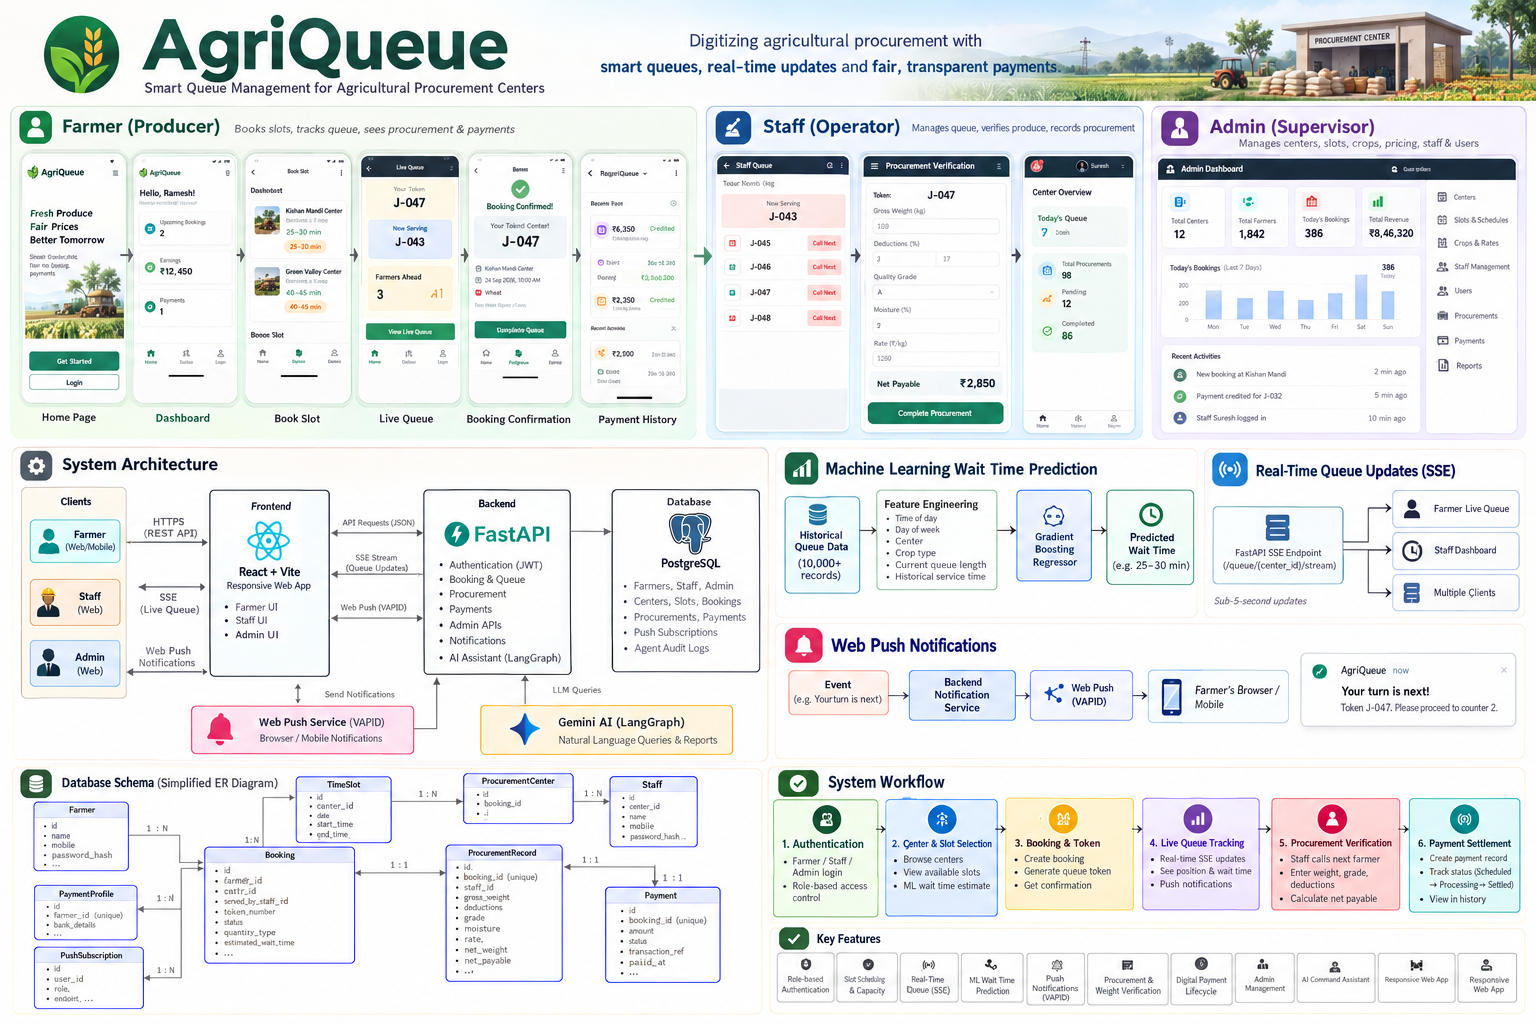
\includegraphics[width=\textwidth]{img/project-overall-image.png}}}
  \caption{AgriQueue Comprehensive Architecture, Module Interfaces, and Operational Workflow}
  \label{fig:project_overall}
\end{figure}

The platform comprises three primary functional pillars:
\begin{itemize}
  \item \textbf{Farmer Module:} Advance slot reservation, digital token generation, live SSE queue monitoring, and transparent payment settlement tracking.
  \item \textbf{Staff Module:} Center-specific queue dispatching, automated weighment entry, moisture deductions, and instant MSP amount computation.
  \item \textbf{Admin Module:} Centralized management of mandis, capacity limits, crop MSP schedules, staff allocations, and dispute resolution.
\end{itemize}

\section{Scope}
\begin{itemize}
  \item \textbf{User roles:} Farmer, Staff (center operator), Admin (government/agency).
  \item \textbf{Produces:} Wheat, Paddy, Cotton, Mustard, Maize, Soybean, Chana, Sugarcane.
  \item \textbf{Queue:} Token-based SSE streaming with 5-second refresh interval.
  \item \textbf{Deployment:} Cloud backend (FastAPI + PostgreSQL), Vercel frontend (React).
  \item \textbf{Out of scope:} Native mobile app, hardware weighbridge integration, SMS gateway.
\end{itemize}

\section{Significance}
\begin{itemize}
  \item Farmers save fuel cost and time by planning visits with advance slot booking.
  \item Procurement centers increase throughput via digital capacity management.
  \item Digital audit trail eliminates manual errors and reduces corruption.
  \item ML analytics enable evidence-based capacity planning for administrators.
  \item Aligns with Government of India's \textbf{Digital India} and \textbf{PM-KISAN} initiatives.
\end{itemize}

\section{Methodology Overview}
\begin{enumerate}
  \item Requirement gathering and stakeholder analysis.
  \item System architecture and database schema design.
  \item Backend API development (FastAPI, SQLAlchemy, asyncpg).
  \item ML model training (HistGradientBoosting on synthetic queue data).
  \item Frontend development (React 19, Vite, custom CSS).
  \item Integration testing -- full farmer-to-payment workflow.
  \item Cloud deployment and production validation.
\end{enumerate}
